\newcommand*\circled[1]{\tikz[baseline=(char.base)]{
		\node[shape=circle,draw,inner sep=2pt] (char) {#1};}}

\section*{H5/6. feladat}
\addcontentsline{toc}{section}{H5/6. feladat}
Határozza meg mekkora fordulatszámon ($\SI{}{1\per\min}$-ban) járhat a légüst nélküli szivattyút hajtó kulisszás hajtómű hajtótengelye, ha a szivattyú $\SI{20}{\celsius}$ hőmérsékletű vizet szállít, hogy a szívócsőben a vízoszlop még éppen ne szakadjon meg! A veszteségeket elhanyagolhatjuk. A $\SI{20}{\celsius}$-hoz tartozó telített gőznyomás

\begin{equation*}
	p_g=\SI{2338}{\Pa},
	\quad
	p_0=\SI{e5}{\Pa},
	\quad
	D=\SI{20}{\centi\meter},
	\quad
	d=\SI{12}{\centi\meter},
	\quad
	s=\SI{25}{\centi\meter},
\end{equation*}
\begin{equation*}
	H=\SI{4}{\meter},
	\quad
	l=\SI{5}{\meter},
	\quad
	\rho_v=\SI{e3}{\kilogram\per\meter\cubed},
	\quad
	g=\SI{9,81}{\meter\per\s\squared}
\end{equation*}
\begin{figure}[h]
	\centering
	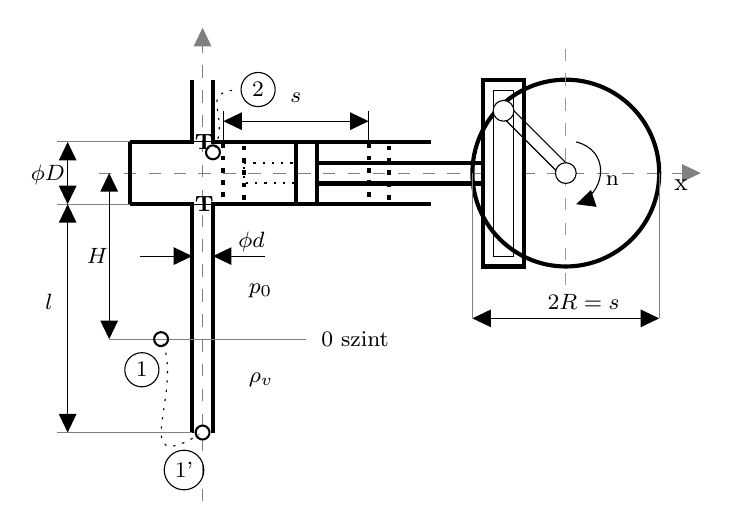
\begin{tikzpicture}[x=0.75pt,y=0.75pt,yscale=-1,xscale=1]
	%uncomment if require: \path (0,300); %set diagram left start at 0, and has height of 300
	
	%Straight Lines [id:da6928752898643067] 
	\draw [color={rgb, 255:red, 128; green, 128; blue, 128 }  ,draw opacity=1 ] [dash pattern={on 4.5pt off 4.5pt}]  (70,80) -- (357,80) ;
	\draw [shift={(360,80)}, rotate = 180] [fill={rgb, 255:red, 128; green, 128; blue, 128 }  ,fill opacity=1 ][line width=0.08]  [draw opacity=0] (8.93,-4.29) -- (0,0) -- (8.93,4.29) -- cycle    ;
	%Straight Lines [id:da3332098294752597] 
	\draw [color={rgb, 255:red, 128; green, 128; blue, 128 }  ,draw opacity=1 ] [dash pattern={on 4.5pt off 4.5pt}]  (120,238) -- (120,13) ;
	\draw [shift={(120,10)}, rotate = 450] [fill={rgb, 255:red, 128; green, 128; blue, 128 }  ,fill opacity=1 ][line width=0.08]  [draw opacity=0] (8.93,-4.29) -- (0,0) -- (8.93,4.29) -- cycle    ;
	%Shape: Right Angle [id:dp6677147550536322] 
	\draw  [line width=1.5]  (115,35) -- (115,65) -- (85,65) ;
	%Shape: Right Angle [id:dp7359276952115859] 
	\draw  [line width=1.5]  (85,95) -- (115,95) -- (115,205) ;
	%Shape: Right Angle [id:dp32949612905558956] 
	\draw  [line width=1.5]  (230,65) -- (125,65) -- (125,35) ;
	%Shape: Right Angle [id:dp9833822872812439] 
	\draw  [line width=1.5]  (125,205) -- (125,95) -- (230,95) ;
	%Straight Lines [id:da331321756527875] 
	\draw [line width=1.5]    (85,65) -- (85,95) ;
	%Straight Lines [id:da5082607934674401] 
	\draw    (115,95) -- (125,95) ;
	%Straight Lines [id:da5767042798474269] 
	\draw    (115,65) -- (125,65) ;
	%Shape: Rectangle [id:dp9462712398642303] 
	\draw  [dash pattern={on 1.69pt off 2.76pt}][line width=1.5]  (130,65) -- (140,65) -- (140,95) -- (130,95) -- cycle ;
	%Shape: Rectangle [id:dp10299731783810784] 
	\draw  [dash pattern={on 0.84pt off 2.51pt}][line width=0.75]  (140,75) -- (165,75) -- (165,85) -- (140,85) -- cycle ;
	%Shape: Rectangle [id:dp26746608188007426] 
	\draw  [dash pattern={on 1.69pt off 2.76pt}][line width=1.5]  (200,65) -- (210,65) -- (210,95) -- (200,95) -- cycle ;
	%Shape: Rectangle [id:dp12515923268225349] 
	\draw  [line width=1.5]  (165,65) -- (175,65) -- (175,95) -- (165,95) -- cycle ;
	%Shape: Rectangle [id:dp40960225950998197] 
	\draw  [line width=1.5]  (175,75) -- (255,75) -- (255,85) -- (175,85) -- cycle ;
	%Shape: Rectangle [id:dp3238526423728385] 
	\draw  [fill={rgb, 255:red, 255; green, 255; blue, 255 }  ,fill opacity=1 ] (260,40) -- (270,40) -- (270,120) -- (260,120) -- cycle ;
	%Shape: Rectangle [id:dp2982134820206286] 
	\draw  [line width=1.5]  (255,35) -- (275,35) -- (275,125) -- (255,125) -- cycle ;
	%Shape: Circle [id:dp7600942698698829] 
	\draw  [line width=1.5]  (250,80) .. controls (250,55.15) and (270.15,35) .. (295,35) .. controls (319.85,35) and (340,55.15) .. (340,80) .. controls (340,104.85) and (319.85,125) .. (295,125) .. controls (270.15,125) and (250,104.85) .. (250,80) -- cycle ;
	%Straight Lines [id:da8743149140372222] 
	\draw [color={rgb, 255:red, 155; green, 155; blue, 155 }  ,draw opacity=1 ] [dash pattern={on 4.5pt off 4.5pt}]  (295,20) -- (295,140) ;
	%Shape: Rectangle [id:dp09029336416708311] 
	\draw   (265,45) -- (300,80) -- (295.76,84.24) -- (260.76,49.24) -- cycle ;
	%Shape: Circle [id:dp9956986330109663] 
	\draw  [fill={rgb, 255:red, 255; green, 255; blue, 255 }  ,fill opacity=1 ] (290,80) .. controls (290,77.24) and (292.24,75) .. (295,75) .. controls (297.76,75) and (300,77.24) .. (300,80) .. controls (300,82.76) and (297.76,85) .. (295,85) .. controls (292.24,85) and (290,82.76) .. (290,80) -- cycle ;
	%Shape: Circle [id:dp9678773828249707] 
	\draw  [fill={rgb, 255:red, 255; green, 255; blue, 255 }  ,fill opacity=1 ] (260,50) .. controls (260,47.24) and (262.24,45) .. (265,45) .. controls (267.76,45) and (270,47.24) .. (270,50) .. controls (270,52.76) and (267.76,55) .. (265,55) .. controls (262.24,55) and (260,52.76) .. (260,50) -- cycle ;
	%Curve Lines [id:da9944157588489633] 
	\draw    (300,65) .. controls (316.05,69.05) and (314.47,87.67) .. (302.62,93.89) ;
	\draw [shift={(300,95)}, rotate = 341.77] [fill={rgb, 255:red, 0; green, 0; blue, 0 }  ][line width=0.08]  [draw opacity=0] (8.93,-4.29) -- (0,0) -- (8.93,4.29) -- cycle    ;
	%Straight Lines [id:da38262917893568904] 
	\draw [color={rgb, 255:red, 128; green, 128; blue, 128 }  ,draw opacity=1 ]   (250,80) -- (250,150) ;
	%Straight Lines [id:da3897224424188508] 
	\draw [color={rgb, 255:red, 128; green, 128; blue, 128 }  ,draw opacity=1 ]   (340,80) -- (340,150) ;
	%Straight Lines [id:da049609724027550595] 
	\draw    (253,150) -- (337,150) ;
	\draw [shift={(340,150)}, rotate = 180] [fill={rgb, 255:red, 0; green, 0; blue, 0 }  ][line width=0.08]  [draw opacity=0] (8.93,-4.29) -- (0,0) -- (8.93,4.29) -- cycle    ;
	\draw [shift={(250,150)}, rotate = 0] [fill={rgb, 255:red, 0; green, 0; blue, 0 }  ][line width=0.08]  [draw opacity=0] (8.93,-4.29) -- (0,0) -- (8.93,4.29) -- cycle    ;
	%Straight Lines [id:da4960904575725176] 
	\draw    (133,55) -- (197,55) ;
	\draw [shift={(200,55)}, rotate = 180] [fill={rgb, 255:red, 0; green, 0; blue, 0 }  ][line width=0.08]  [draw opacity=0] (8.93,-4.29) -- (0,0) -- (8.93,4.29) -- cycle    ;
	\draw [shift={(130,55)}, rotate = 0] [fill={rgb, 255:red, 0; green, 0; blue, 0 }  ][line width=0.08]  [draw opacity=0] (8.93,-4.29) -- (0,0) -- (8.93,4.29) -- cycle    ;
	%Straight Lines [id:da3799217778581234] 
	\draw    (200,50) -- (200,65) ;
	%Straight Lines [id:da7818492293054387] 
	\draw    (130,50) -- (130,65) ;
	%Straight Lines [id:da5925451459425932] 
	\draw [color={rgb, 255:red, 128; green, 128; blue, 128 }  ,draw opacity=1 ]   (85,65) -- (50,65) ;
	%Straight Lines [id:da411352935885561] 
	\draw [color={rgb, 255:red, 128; green, 128; blue, 128 }  ,draw opacity=1 ]   (85,95) -- (50,95) ;
	%Straight Lines [id:da13875478110648243] 
	\draw    (55,92) -- (55,68) ;
	\draw [shift={(55,65)}, rotate = 450] [fill={rgb, 255:red, 0; green, 0; blue, 0 }  ][line width=0.08]  [draw opacity=0] (8.93,-4.29) -- (0,0) -- (8.93,4.29) -- cycle    ;
	\draw [shift={(55,95)}, rotate = 270] [fill={rgb, 255:red, 0; green, 0; blue, 0 }  ][line width=0.08]  [draw opacity=0] (8.93,-4.29) -- (0,0) -- (8.93,4.29) -- cycle    ;
	%Straight Lines [id:da1962128166500996] 
	\draw    (150,120) -- (128,120) ;
	\draw [shift={(125,120)}, rotate = 360] [fill={rgb, 255:red, 0; green, 0; blue, 0 }  ][line width=0.08]  [draw opacity=0] (8.93,-4.29) -- (0,0) -- (8.93,4.29) -- cycle    ;
	%Straight Lines [id:da17976486405599967] 
	\draw    (90,120) -- (112,120) ;
	\draw [shift={(115,120)}, rotate = 180] [fill={rgb, 255:red, 0; green, 0; blue, 0 }  ][line width=0.08]  [draw opacity=0] (8.93,-4.29) -- (0,0) -- (8.93,4.29) -- cycle    ;
	%Straight Lines [id:da3832087653428644] 
	\draw [color={rgb, 255:red, 128; green, 128; blue, 128 }  ,draw opacity=1 ]   (75,160) -- (170,160) ;
	%Straight Lines [id:da42088226594876965] 
	\draw    (75,157) -- (75,83) ;
	\draw [shift={(75,80)}, rotate = 450] [fill={rgb, 255:red, 0; green, 0; blue, 0 }  ][line width=0.08]  [draw opacity=0] (8.93,-4.29) -- (0,0) -- (8.93,4.29) -- cycle    ;
	\draw [shift={(75,160)}, rotate = 270] [fill={rgb, 255:red, 0; green, 0; blue, 0 }  ][line width=0.08]  [draw opacity=0] (8.93,-4.29) -- (0,0) -- (8.93,4.29) -- cycle    ;
	%Straight Lines [id:da4079808873067292] 
	\draw [color={rgb, 255:red, 128; green, 128; blue, 128 }  ,draw opacity=1 ]   (50,205) -- (115,205) ;
	%Straight Lines [id:da9343602687602341] 
	\draw    (55,202) -- (55,98) ;
	\draw [shift={(55,95)}, rotate = 450] [fill={rgb, 255:red, 0; green, 0; blue, 0 }  ][line width=0.08]  [draw opacity=0] (8.93,-4.29) -- (0,0) -- (8.93,4.29) -- cycle    ;
	\draw [shift={(55,205)}, rotate = 270] [fill={rgb, 255:red, 0; green, 0; blue, 0 }  ][line width=0.08]  [draw opacity=0] (8.93,-4.29) -- (0,0) -- (8.93,4.29) -- cycle    ;
	%Curve Lines [id:da9010122588735285] 
	\draw [color={rgb, 255:red, 0; green, 0; blue, 0 }  ,draw opacity=1 ] [dash pattern={on 0.84pt off 2.51pt}]  (100.98,162.24) .. controls (110.29,186.54) and (84.11,226.42) .. (118.39,205.98) ;
	\draw [shift={(120,205)}, rotate = 328.34] [color={rgb, 255:red, 0; green, 0; blue, 0 }  ,draw opacity=1 ][line width=0.75]      (0, 0) circle [x radius= 3.35, y radius= 3.35]   ;
	\draw [shift={(100,160)}, rotate = 63.43] [color={rgb, 255:red, 0; green, 0; blue, 0 }  ,draw opacity=1 ][line width=0.75]      (0, 0) circle [x radius= 3.35, y radius= 3.35]   ;
	%Curve Lines [id:da3487325984899232] 
	\draw  [dash pattern={on 0.84pt off 2.51pt}]  (126.09,67.66) .. controls (132.79,51.45) and (118.92,42.23) .. (135,40) ;
	\draw [shift={(125,70)}, rotate = 297.42] [color={rgb, 255:red, 0; green, 0; blue, 0 }  ][line width=0.75]      (0, 0) circle [x radius= 3.35, y radius= 3.35]   ;
	
	% Text Node
	\draw (115,90) node [anchor=north west][inner sep=0.75pt]   [align=left] {\textbf{{\footnotesize T}}};
	% Text Node
	\draw (115,60) node [anchor=north west][inner sep=0.75pt]   [align=left] {\textbf{{\footnotesize T}}};
	% Text Node
	\draw (346,82) node [anchor=north west][inner sep=0.75pt]  [font=\footnotesize] [align=left] {{\small x}};
	% Text Node
	\draw (313,80) node [anchor=north west][inner sep=0.75pt]  [font=\footnotesize] [align=left] {{\footnotesize n}};
	% Text Node
	\draw (285,137) node [anchor=north west][inner sep=0.75pt]  [font=\footnotesize] [align=left] {{\footnotesize $2R=s$}};
	% Text Node
	\draw (161,40) node [anchor=north west][inner sep=0.75pt]  [font=\footnotesize] [align=left] {{\footnotesize $s$}};
	% Text Node
	\draw (36,75) node [anchor=north west][inner sep=0.75pt]  [font=\footnotesize] [align=left] {{\footnotesize $\phi D$}};
	% Text Node
	\draw (136,107) node [anchor=north west][inner sep=0.75pt]  [font=\footnotesize] [align=left] {{\footnotesize $\phi d$}};
	% Text Node
	\draw (176,155) node [anchor=north west][inner sep=0.75pt]  [font=\footnotesize] [align=left] {{\footnotesize 0 szint}};
	% Text Node
	\draw (63,115) node [anchor=north west][inner sep=0.75pt]  [font=\footnotesize] [align=left] {{\footnotesize $H$}};
	% Text Node
	\draw (43,137) node [anchor=north west][inner sep=0.75pt]  [font=\footnotesize] [align=left] {{\footnotesize $l$}};
	% Text Node
	\draw (81,165) node [anchor=north west][inner sep=0.75pt]  [font=\footnotesize] [align=left] {{\footnotesize \circled{1}}};
	% Text Node
	\draw (100,212) node [anchor=north west][inner sep=0.75pt]  [font=\footnotesize] [align=left] {{\footnotesize \circled{1'}}};
	% Text Node
	\draw (137,30) node [anchor=north west][inner sep=0.75pt]  [font=\footnotesize] [align=left] {{\footnotesize \circled{2}}};
	% Text Node
	\draw (141,175) node [anchor=north west][inner sep=0.75pt]  [font=\footnotesize] [align=left] {{\footnotesize $\rho_v$}};
	% Text Node
	\draw (141,132) node [anchor=north west][inner sep=0.75pt]  [font=\footnotesize] [align=left] {{\footnotesize $p_0$}};
	
	\end{tikzpicture}
\end{figure}

Instacionárius áramlásról lévén szó, az áramvonal (1-2) pontjaira felírható Bernoulli-egyenlet a következő:
\begin{equation*}
	\int_{1}^{2}{\frac{\delta v}{\delta t}\cdot ds + \left[{\frac{v^2}{2} + U + \frac{p}{\rho}}\right]_1^2}=0
\end{equation*}
Az áramvonal két pontjában az összetartozó adatok:
\begin{center}
	\begin{tabular}{ll}
		\circled{1} pont & \circled{2} pont \\
		$v_1=0$ & $v_2=0$ \\
		$p_1=p_0$ & $p_2=p_g$ \\
		$U_1=0$ & $U_2=gH$
	\end{tabular}
\end{center}
Az egyenlet első tagját vizsgálva, annak integrálása szakaszonként elvégezhető:
\begin{equation*}
	\int_{1}^{1'}{\frac{\delta v}{\delta t}\cdot ds = 0};
	\int_{1'}^{2'}{\frac{\delta v}{\delta t}\cdot ds = a\cdot L};
	\int_{2'}^{2}{\frac{\delta v}{\delta t}\cdot ds = a_{max}\cdot 1}
\end{equation*}
A fentiek alapján a Bernoulli-egyenlet a következőképp írható:
\begin{equation*}
	a\cdot L+a_{max}\cdot 1+\frac{p_g}{\rho}-\frac{p_0}{\rho}+g\cdot H = 0
\end{equation*}
A kontinuitás a gyorsulásokra is érvényes:
\begin{equation*}
	a\cdot A_1 = a_{max}\cdot A_2 \rightarrow a=a_{max}\cdot\frac{A_2}{A_1}
\end{equation*}
ezzel:
\begin{equation*}
	a_{max}\cdot\left(\frac{A_2}{A_1}\cdot L+1\right)=\frac{1}{\rho}\left(p_0-p_g\right)-gH
\end{equation*}
Ebből a gyorsulás megengedhető maximális értéke:
\begin{equation*}
	\bold{a_{max}} \le \frac{ \frac{1}{\rho} \left( p_0-p_g \right) -g\cdot H }{ \frac{A_2}{A_1} \cdot L+1 } = \frac{ \frac{1}{10^3}\left( 10^5 -2338 \right) - 9,81 \cdot 4}{\left(\frac{20}{12}\right)^2 \cdot 5} \le \SI{4,206}{\left(\meter\per\sec\squared\right)}
\end{equation*}
A fordulatszám pedig: \(a=r\cdot \omega^2=4\cdot r\cdot \pi^2 \cdot n^2\)-ből:
\begin{equation*}
	\bold{n} = \left[ \frac{a}{4 \cdot r \cdot \pi ^2} \right]^\frac{1}{2}=\left[ \frac{4,206}{4 \cdot 0,125 \cdot \pi^2} \right]^\frac{1}{2}=\SI{0,92}{\left(1\per\sec\right)} \rightarrow \SI{55,2}{\left(1\per\min\right)}
\end{equation*}
ahol
\begin{equation*}
	\frac{A_2}{A_1}=\left( \frac{D}{d} \right)^2=\left( \frac{20}{12} \right)^2 
\end{equation*}